\documentclass{article}
\usepackage{graphicx}

\begin{document}

\title{11791 - Homework 1 - Named Entity Recognition Implementation with UIMA SDK}
\author{Mohammad Gowayyed \\ mgowayye@andrew.cmu.edu}

\maketitle
\begin{abstract}
In this document, I report briefly my implementation for a gene named entity recognition. I used the algorithm described in \cite{banner} and used some of the published implementation at \cite{banner_code}. Whenever I use any of their code, I am clearly stating this within my Java code.
\end{abstract}


\section{Design}
\subsection{Architecture}

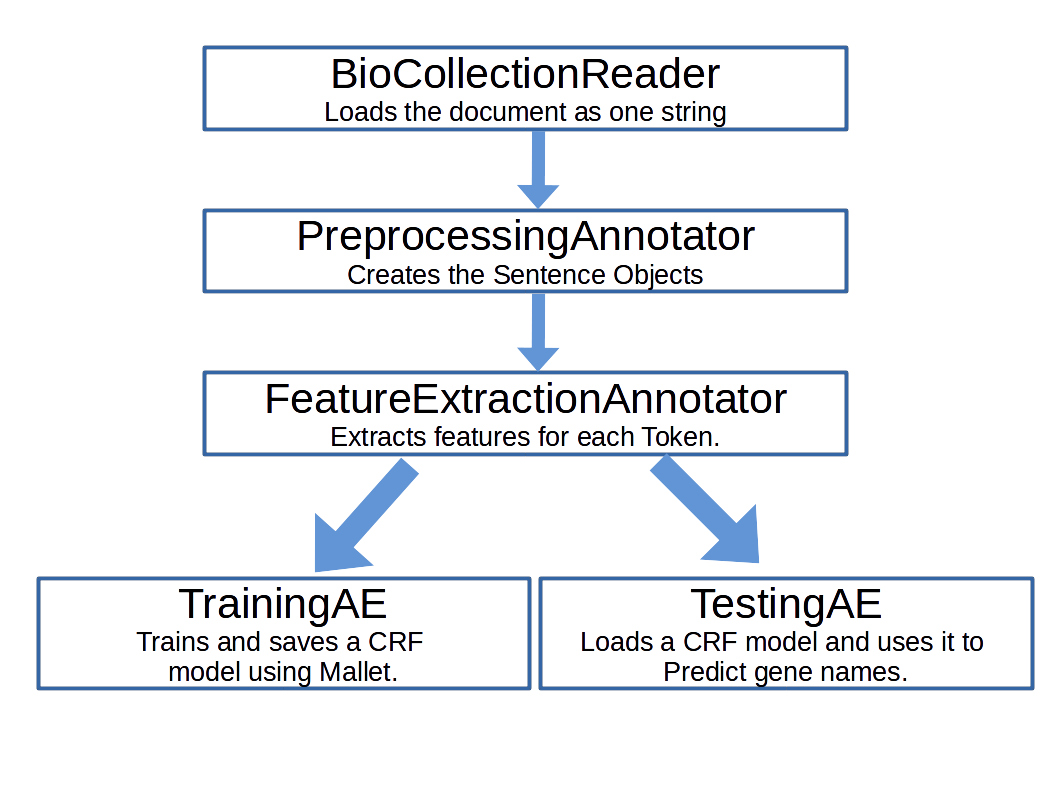
\includegraphics[width=14cm]{framework.png}

\subsection{Data Flow}

\section{Domain diagram for IntelligentInformationSystem}

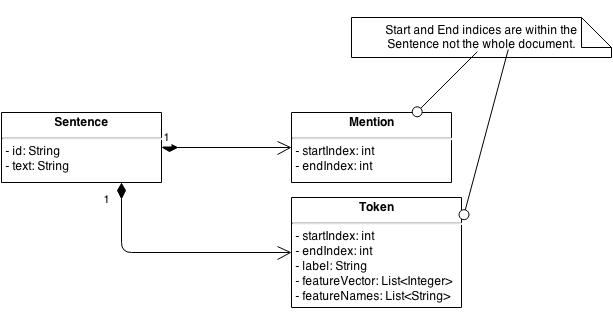
\includegraphics[width=14cm]{HW1-genes-UML.png}


\begin{thebibliography}{9}


\bibitem{banner}
BANNER: an executable survey of advances in biomedical named entity recognition,
Leaman, Robert and Gonzalez, Graciela and others,
  Pacific Symposium on Biocomputing,
  2008

\bibitem{banner_code}
  http://banner.sourceforge.net/

\end{thebibliography}
\end{document}